%% Los cap'itulos inician con \chapter{T'itulo}, estos aparecen numerados y
%% se incluyen en el 'indice general.
%%
%% Recuerda que aqu'i ya puedes escribir acentos como: 'a, 'e, 'i, etc.
%% La letra n con tilde es: 'n.


\chapter{Introducción}

A lo largo de la historia de la agricultura, el hombre ha desarrollado el mejoramiento vegetal en forma sistemática y lo ha convertido en un instrumento esencial para incrementar la producción agrícola en términos de cantidad, calidad y diversidad. Las variedades mejoradas son el resultado del trabajo llevado a cabo en los programas de fitomejoramiento, los cuales se extienden a lo largo de varios años y requieren cuantiosas inversiones. En etapas avanzadas de estos programas, comúnmente se llevan a cabo ensayos multiambientales (EMA) de comparación de rendimientos, donde un conjunto de variedades se evalúan en múltiples ambientes. Estos son esenciales debido a la presencia de interaccion genotipo - ambiente (IGA) la cual es inevitable debido a las variaciones en las condiciones climáticas y de suelo de los distintos ambientes analizados. La IGA es considerada casi unánimemente por los fitomejoradores como el principal factor que limita la selección de cultivares superiores y, en general, afecta la eficiencia de los programas de mejoramiento \citep{Crossaetal1990, CruzMedina1992}; \textbf{Kang y Magari, 1996)}. Cuando los ambientes son muy diferentes, la IGA usualmente gana importancia porque cambian el rango de las líneas de mejoramiento. \citet{GauchZobel1997} explicaron que si no hubiera interacción, una sola variedad o híbrido rendirían al máximo en todo el mundo, además los materiales podrían evaluarse en un solo lugar y proporcionarían resultados universales.


\textbf{Peto (1982)} ha distinguido las interacciones cuantitativas, conocidas también como sin cambio de rango o \emph{no crossover} (NCOI), de las cualitativas, denominadas a su vez como con
cambio de rango o \emph{crossover} (COI) (Cornelius et al., 1996). Cuando dos genotipos X e Y tienen una respuesta diferencial en dos ambientes, se dice que la IGA es del tipo COI si hay cambios en el orden de los genotipos según su rendimiento (Figura \ref{fig:fig11}(A)) y del tipo NCOI si su ordenamiento permanece sin cambios (Figura  \ref{fig:fig11}(B)). Por otro lado, se dice que la IGA es inexistente cuando los genotipos responden de manera similar en ambos ambientes (Figura \ref{fig:fig11}(C)). 


\begin{figure}[h]
\begin{center}
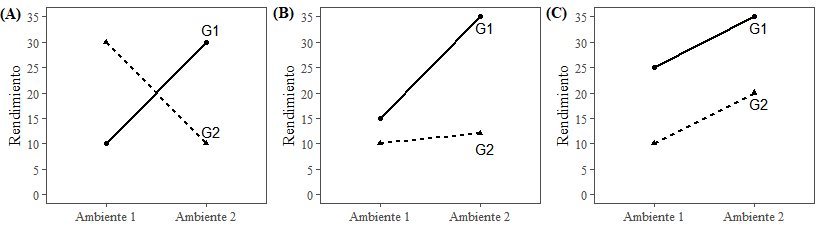
\includegraphics[width=14cm]{./Graficos/interac}
\end{center}
\caption{Representación gráfica de tipos de IGA: (A)IGA crossover, (B) IGA no crossover y (C) no IGA}
\label{fig:fig11}
\end{figure}


Entre las implicancias negativas de la IGA en los programas de mejoramiento se encuentra el impacto negativo sobre la heredabilidad, cuanto menor sea la heredabilidad de un caracter, mayor será la dificultad para mejorarlo. Como consecuencia, la información sobre la estructura y la naturaleza de la IGA es particularmente útil para determinar si se deben desarrollar cultivares con adaptación amplia o específica (\textbf{Bridges, 1989}). Conceptos importantes tales como regiones ecológicas, ecotipos, mega-ambientes, adaptación especifica y estabilidad se pueden analizar a partir de la IGA (Yan y Hunt, 2001).

Un análisis adecuado de la información de los EMA es indispensable para el éxito del programa de mejoramiento genético de los cultivos. El rendimiento medio en los ambientes es un indicador suficiente del rendimiento genotípico sólo en ausencia de IGA \citep{YanKang2003}. Sin embargo, la aparición de IGA es inevitable y no basta con la comparación de las medias de los genotipos, sino que se debe recurrir a una metodología estadística más aporopiada. Las más difundidas para analizar los datos provenientes de EMA se basan en modificaciones de los modelos de regresión, análisis de variancia (ANOVA) y técnicas de análisis multivariado. 

Particularmente, para el estudio de la IGA y los análisis que de ella se derivan, dos modelos multiplicativos han aumentado su popularidad entre los fitomejoradores como herramientas de análisis gráfico: el modelo de los efectos principales aditivos e interacción multiplicativa (\emph{Additive Main effects and Multiplicative Interaction}, AMMI) \citep{Kempton1984,Gauch1988} y el de regresión por sitio (\emph{Site Regression model}, SREG) (\textbf{Cornelius et al., 1996}; \citep{GauchZobel1997}. En su forma regular, AMMI explora la matriz de IGA realizando una descomposición en valores singulares (DVS) sobre la matriz residual de un ANOVA que considera el efecto aditivo de los genotipos (G) y ambientes (A). Mientras que, en SREG el ANOVA sólo incluye el efecto de A, lo que permite analizar G e IGA en forma conjuntamente. El resultado de los dos primeros términos multiplicativos de la DVS a menudo se presentan en un biplot llamado GE para el modelo AMMI y GGE para SREG (\textbf{Yan y Hunt (2002)}). Sin embargo, estos modelos no siempre son lo suficientemente eficiente para analizar la estructura de datos MET de programas de mejoramiento vegetal. Por un lado, tiene serias limitaciones frente a información faltante y, apesar de que los MET están diseñados para que todos los genotipos se evalúen en todos los ambientes, la presencia de valores perdidos es muy común. Esto ocurre, por ejemplo, debido a errores de medición o pérdidas de plantas por presencia de animales, inundaciones o problemas durante la cosecha, además de la dinámica propia de la evaluaciones en las que se incorporan y se descartan genotipos debido a su pobre desempeño (Hill y Rosemberg, 1985). Numerosas metodologías de imputación se han estado desarrollando en los ultimos años para solventar esta limitación (CITAS.......). Por otro lado, son sensibles a la presencia de observaciónes atipicas, lo cual es una regla más que una excepción cuando se consideran datos reales. Para superar esta fragilidad, recientemente distintas metodologias robustas se han desarrollado para el modelo AMMI (Rodrigues et al. (2015)). 


En este contexto, el análisis de datos provenientes de EMA requiere metodología estadística cuyas rutinas informáticas no se encuentran disponibles en programas comerciales debido a su reciente desarrollo o bien se deben utilizar varios de ellos para lograr un único objetivo. Esto último genera el inconveniente de tener que disponer de todos los programas necesarios para los distintos análisis, atender los requerimientos de formatos de datos usados por cada uno de ellos, y comprender los diversos tipos de salidas en las que se presentan los resultados obtenidos. Además, los costos de las licencias algunos programas pueden resultar muy elevados. 

Ante estas dificultades, una alternativa para el análisis es el empleo de algún lenguaje de programación de distribución libre y gratuita, que le confiera al analista la flexibilidad necesaria para cumplir con su objetivo. En este contexto, R es uno de los lenguajes de programación desarrollados para el análisis de datos de mayor uso en la actualidad. R es un software de uso libre y distribuido bajo los términos de la \emph{General Public Licence} (GNU). Este programa se descarga de un repositorio mantenido por \emph{The R Foundation for Statistical Computing} conocido como CRAN (\emph{Comprehensive R Archive Network}), en el cual también se encuentran disponibles miles de paquetes adicionales que consisten en conjuntos de funciones desarrolladas con fines específicos que se distribuyen con un protocolo determinado, garantizando su correcto funcionamiento. Cualquier desarrollador puede producir su propio paquete y publicarlo en CRAN, siempre que cumpla con los requisitos establecidos y pase correctamente por los procedimientos de control. Además, hay paquetes que pueden obtenerse de otros repositorios como Github, Bioconductor, rOpenSci, entre otros. R es propicio para el análsis de datos de EMA puesto que se ha desarrollado metodología específica para este entorno computacional. 

A pesar de estas ventajas, el análisis de datos de EMA en R presenta algunos desafíos. Por un lado, existen numerosos paquetes con funcionalidad afín que hay que identificar cómo combinar adecuadamente. Por otro lado, el software puede resultar dificultoso para aquellos analistas no familiarizados con la programación. Atendiendo a estas dos necesidades, se crea un paquete que reuna las funciones más útiles y ofrece otras nuevas recientemente disponible en la literatura a fin de solventar la primera de ellas. Para la segunda, se crea una aplicación web Shiny de libre acceso mediante conexión a internet. 
